\section{Работа с лабораторной установкой <<Microcode>>}
\label{s::ch::practice::software}

Цель лабораторной установки <<Microcode>> --- закрепление теоретических основ реализации арифметических операций.

Поставленная цель достигается за счет того, что:
\begin{itemize}
    \item предлагается готовая операционная часть устройства (см. рисунок \ref{fig::ch::practice::model} и теорию в разделе \ref{ch::practice}), в структуре которой требуется разобраться и понять, как имеющимися средствами решить задачу (т.е. выполнить некоторую арифметическую операцию);

    \item моделируется работа центрального управляющего устройства, которое выдает задание и принимает результаты по определенным правилам;

    \item <<Microcode>> позволяет студенту задать собственные входные данные и выполнить пошаговое управление в режиме отладки;
    
    \item <<Microcode>> автоматически выполняет многократное тестирование правильности решения задачи по методу <<черного ящика>>;
    
    \item выполняемые <<Microcode>> тесты покрывают все ветки правильного алгоритма решения задачи (арифметической операции);
    
    \item тесты покрытия создаются <<Microcode>> на основе генератора случайных чисел;
    
    \item в <<Microcode>> заложена возможность генерации индивидуальных вариантов заданий, создаваемых за счет перестановки индексов управляющих сигналов $y$, что порождает $n!$ возможных уникальных вариантов кодирования, при среднем $n\ge 12$;
    
    \item в диалогах <<Microcode>> для ввода отладочных данных автоматически рассчитывается результат, а также выводятся десятичные представления числовых операндов, что дает возмножность глубже разобраться в форматах и кодах.
\end{itemize}


\subsection{Принципы работы <<Microcode>>}

Лабораторная установка <<Microcode>> позволяет загружать групу заданий. Например, в рамках одной группы могут быть загружены задания на умножение чисел различными способами (см. рисунок \ref{fig:mic:MicWindow}).

\begin{figure}
    \centering
    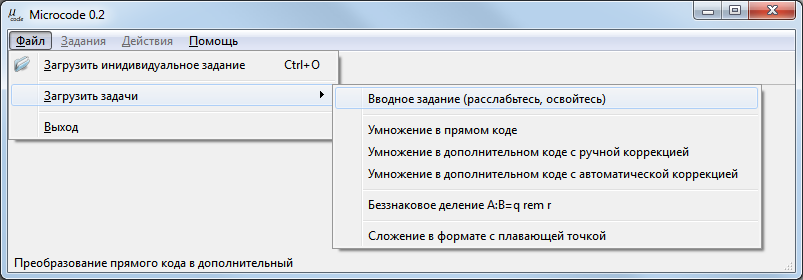
\includegraphics[width=\textwidth]{fig/MicWindow}
    \caption{Главное окно <<Microcode>> (русский язык интерфейса)}\label{fig:mic:MicWindow}
\end{figure}

Отдельное задание представляет собой вычислительное устройство, постороенное в соответствии с принципами, изложенными в разделе \ref{ch::practice} и способное выполнять ту или иную сложную вычислительную операцию, например, умножение или деление.

Пользователю предлагается готовая схема операционной части, в устройстве и назначении которой он должен разобраться, опираясь на изученную теорию. В распоряжении пользователя имеется набор управляющих сигналов, с помощью которых он может изменять состояние операционной части. Задача пользователя --- реализовать алгоритм работы сложной вычислительной операции.

У пользователя имеются следующие возможности реализовать алгоритм работы устройства:
\begin{itemize}
    \item вручную выполнить выдачу необходимых управляющих сигналов, предварительно задав наборы управляющих сигналов в ПЗУ микрокоманд;
    \item запрограммировать автомат Мили или Мура, заполнив таблицу ПЗУ микропрограмм.
\end{itemize}

Все значения в таблицы ПЗУ заносятся в шестнадцатеричной системе счисления. Управляющие сигналы кодируются двоичным вектором, который в ПЗУ вносится в шестнадцатеричном представлении, например, если требуется выдать сигналы $y_5,y_3,y_2,y_0$, то в соответствующей ячейке ПЗУ нужно записать значение \Machine{0x2D}.

По команде пользователя <<Microcode>> выполняет автоматическое тестирование составленного пользователем алгоритма. Чтобы составить корректный алгоритм, пользователь может использовать специальный режим отладки, в котором он может задать исходные данные и в пошаговом режиме отследить изменения, происходящие в операционной части.

Прохождение автоматических тестов является допуском к защите разультатов работы.


\subsection{Задания на лабораторные работы}

В рамках лабораторной работы студент выполняет задание, которое выдает преподаватель.

В лабораторной установке <<Microcode>> реализованы следующие задания: 
\begin{itemize}
    \item перевод прямого кода в дополнительный;
    \item умножение в прямом коде;
    \item умножение в дополнительном коде с ручной коррекцией;
    \item умножение в дополнительном коде с автоматической коррекцией;
    \item беззнаковое деление $A\div B = \DivAnswer{q}{r}$;
    \item сложение в формате с плавающей точкой.
\end{itemize}


\subsection{Выполнение задания}

После выбора группы заданий, становится активным пункт меню <<Задания>>(<<Tasks>>), позволяющий переключаться между заданиями в рамках группы (см. рисунок \ref{fig:mic:MicTaskWindow}). Менять группу заданий в дальнейшем нельзя.

\begin{figure}
    \centering
    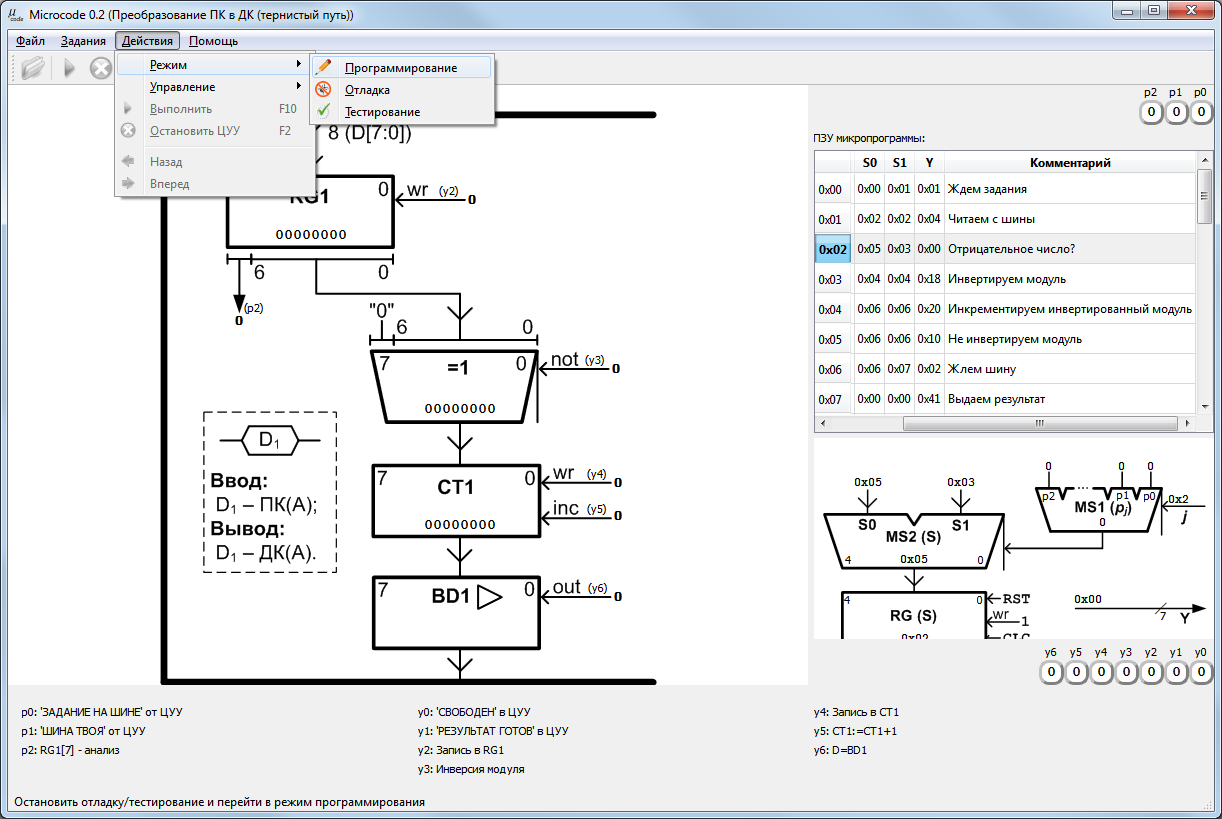
\includegraphics[width=\textwidth]{fig/MicTaskWindow}
    \caption{<<Microcode>> после загрузки заданий}\label{fig:mic:MicTaskWindow}
\end{figure}

Пункт меню <<Действия>> позволяет выполнить те или иные действия в текущем задании:
\begin{itemize}
    \item выбрать один из режимов работы: <<Программирование>> (
\includegraphics[width=16pt]{fig/microcode/image/programming.png}), <<Отладка>> (
\includegraphics[width=16pt]{fig/microcode/image/debug.png}) или <<Тестирование>> (
\includegraphics[width=16pt]{fig/microcode/image/autotest.png});
    \item выбрать управление: <<Ручное>> (
\includegraphics[width=16pt]{fig/microcode/image/manualgun.png}), 
                              <<Автомат Мили>> (
\includegraphics[width=16pt]{fig/microcode/image/miligun.png})
                              или <<Автомат Мура>> (
\includegraphics[width=16pt]{fig/microcode/image/mooregun.png});
    \item выполнять/останавливать шаги отладки или автотесты;
    \item перемещаться в отладочном режиме по истории тактов.
\end{itemize}

Режим работы <<Программирование>> (<<Programming>>) предназначен для редактирования ПЗУ управляющей части. Как только редактирование ячейки ПЗУ завершается, соответствующие управляющие сигналы распространаяются по схеме, но ошибки управления не выдаются, даже если они есть.

Режим <<Отладка>> (<<Debug>>) предназначен для пошагового выполнения придуманного студентом алгоритма управления. В момент переключения в этот режим студенту предлагается ввести исходные данные. После того, как данные будут введены, <<Microcode>> переключается в пошаговый (потактный) режим тестирования. В случае ручного управления (<<Управление/Ручное>> (<<MCU/Manual>>)) пользователь выбирает в таблице <<ПЗУ микрокоманд>> строку с нужной командой и нажимает кнопку <<Выполнить>> (<<Execute>>) или горячую клавишу <<F10>>, что приводит к переключению в следующий такт. В случае автоматического управления (<<Aвтомат Мили>> (<<Mili>>), <<Автомат Мура>> (<<Moore>>)) текущая ячейка ПЗУ микропрограммы (строка таблицы) подсвечивается. Если в процессе выполнения теста фиксируется ошибка, то тестирование прекращается, выводится соответствующее сообщение, и выполняется переход в режим программирования. Если алгоритм выполнен безошибочно и в ЦУУ корректно выдан правильный результат, то выводится информационное сообщение об успешном прохождении отладочного теста.

В режиме <<Тестирование>> (<<Autotest>>) выполняется тестирование на случайным образом генерируемых входных данных. Состояние операционной части при этом не отображается. При ручном управлении автотесты выполняются в пошаговом режиме, в противном случае --- в автоматическом.

В режимах отладки и тестирования фиксируются следующие ошибки, приводящие к прекращению теста:
\begin{itemize}
    \item выполняется чтение данных с <<пустой>> шины;
    \item выполняется выдача данных на <<занятую>> шину;
    \item нарушается протокол взаимодействия с ЦУУ, например, до выдачи результата, выдается сигнал <<Свободен>>;
    \item выдаются конфликтующие сигналы управления элементом памяти, например на регистр одновременно подаются управляющие сигналы сдвига и сброса.
\end{itemize}

Чтобы считать операнды, требуется выполнить следующие действия.
\begin{itemize}
    \item Выдавать сигнал <<Свободен>> ($y_0$, $Y=\Machine{0x0001}$) в течение некоторого числа тактов (не более 6), пока осведомительный сигнал <<Задание на шине>> ($p_0$) не установится в 1.
    \item Сигнал <<Задание на шине>> выдается ЦУУ в течение одного такта, в этом такте также нужно выдавать сигнал <<Свободен>>.
    \item ЦУУ, в течение одного или нескольких тактов, следующих после такта, в котором выдавался сигнал <<Задание на шине>> выдает на шину фрагменты задания. Необходимо считать эти фрагменты в регистры.
\end{itemize}

Чтобы выдать результат, требуется выполнить следующие действия.
\begin{itemize}
    \item Выдавать сигнал <<Результат готов>> ($y_1$, $Y=\Machine{0x0002}$) в течение некоторого числа тактов (не более 6), пока осведомительный сигнал <<Шина твоя>> ($p_0$) не установится в 1.
    \item Сигнал <<Шина твоя>> выдается ЦУУ в течение одного такта, в этом такте также нужно выдавать сигнал <<Результат готов>>.
    \item В течение одного или нескольких тактов, следующих после такта, в котором выдавался сигнал <<Шина твоя>> следует в определенном в задании порядке выдавать фрагменты результата на шину.
\end{itemize}


Результатом работы являются заполненные ПЗУ микрокоманд (ПЗУ микропрограмм). Допуском к защите результатов работы является успешное прохождение студентом отладочных или автоматических тестов.


\subsection{Генерация индивидуальных вариантов заданий}

С помощью microcode можно сгенерировать индивидуальные варианты для каждого студента. Для этих целей нужно сформировать специальный текстовый файл, содержащий список адресатов\footnote{Тех, для кого предназначены индивидуальные варианты заданий. Т.е. студентов.} в формате JSON\footnote{JSON --- JavaScript Object Notation.  Текстовый формат обмена данными, основанный на JavaScript. Прост и лаконичен. Как и многие другие текстовые форматы, JSON легко читается людьми. Формат был разработан Дугласом Крокфордом.}. Файл должен быть сохранен в кодировке UTF-8 и может быть создан в любом подходящем текстовом редакторе.

JSON-содержимое файла адресатов представляет собой массив объектов, состоящих из двух строковых атрибутов:
\begin{itemize}
    \item \verb"id" --- строка, идентифицирующая студента, как правило, содержащая Ф.И.О. студента;
    \item \verb"secret_prefix" --- секретная информация\footnote{В зависимости от степени параноидальности преподавателя, может быть как случайной последовательностью, так и вполне предсказуемой по некоторому, известному только преподавателю, правилу, например, фамилия студента на латинице, или его Ф.И.О., или первые три буквы фамилии\ldots}.
\end{itemize}

Пример содержимого файла адресатов:
\begin{verbatim}
[
    {   "id": "Иванов И.И.",
        "secret_prefix": "IvanovSecret"},
        
    {   "id": "Петров П.П.",
        "secret_prefix": "PetrovSecret"},
        
    {   "id": "Сидоров С.С.",
        "secret_prefix": "SidorovSecret"}
]
\end{verbatim}

После того, как файл подготовлен, можно сгенерировать с помощью microcode индивидуальные варианты. Для этого выполняется пункт меню <<Файл/Создать индивидуальные варианты\ldots>> (<<File/Create individual vatiants\ldots>>). В появившемся диалоге (см. рисунок \ref{fig:mic:genvariants}) следует заполнить необходимые поля.
\begin{itemize}
    \item <<Секрет>>(<<The secret:>>) --- секретная информация, которая используется для проверки подлинности индивидуального варианта. Описание проверки подлинности приводится в разделе \ref{ss:mic:check}.
    
    \item <<Файл с адресатами:>>(<<The recipients file:>>) --- путь к подготовленному файлу адресатов.
    
    \item <<Варианты в папку:>>(<<Variants folder:>>) --- каталог, в котором будут созданы файлы индивидуальных вариантов. Имена файлов будут совпадать со значением атрибута \verb"id" в файле адресатов и иметь расширение <<*.json>>.
\end{itemize}

\begin{figure}[!ht]
    \centering
    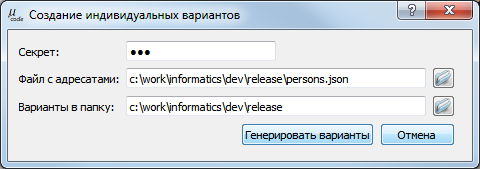
\includegraphics{fig/micvariants}
    \caption{Диалог <<Microcode>> для генерации индивидуальных вариантов (русский язык интерфейса)}\label{fig:mic:genvariants}
\end{figure}

Например, если загрузить приведенный выше файл адресатов, и в качестве секрета ввести <<123>>, то для Иванова будет сгенерирован текстовый файл <<Иванов И.И..json>> со следующим JSON-содержимым:

\begin{verbatim}
{
  "id": "Иванов И.И.",
  "signature": "673e420b...8e76eff8",
  "swap_history": "783590fc...e1c54474"
}
\end{verbatim}

Этот файл может быть загружен в microcode и управляющие сигналы будут перетасованы.


\subsection{Загрузка индивидуального варианта}

После того, как файлы индивидуальных заданий сгенерированы их следует раздать студентам. Индивидуальный вариант загружается студентом командой меню <<Файл/Открыть индивидуальный вариант\ldots>>(<<File/Open individual variant\ldots>>).


\subsection{Проверка подлинности индивидуального варианта}
\label{ss:mic:check}

Файл индивидуального варианта защищен криптографически. Чтобы выполнить проверку подлинности варианта, необходимо выполнить команду меню <<Файл/Проверить индивидуальный вариант\ldots>>(<<File/Validate individual variant\ldots>>).

В диалоге проверки варианта (см. рисунок \ref{fig:mic:checkvarian}) следует ввести конкатенацию секретов $s_1s_2$, где $s_1$ --- секрет, указанный в поле \verb"secret_prefix" файла адресатов, а $s_2$ --- секрет, заданный в диалоге генерации вариантов (см. рисунок \ref{fig:mic:genvariants}).

Для Иванова в приводимых примерах следует ввести: <<IvanovSecret123>>.

\begin{figure}[!ht]
    \centering
    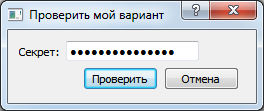
\includegraphics{fig/checkvarian}
    \caption{Диалог <<Microcode>> для проверки подлинности индивидуального варианта (русский язык интерфейса)}\label{fig:mic:checkvarian}
\end{figure}

Без знания секрета, разделенного на две части --- персональную и общую, подделка задания представляет собой вычислительно сложную задачу.

\subsection{Защита результатов работы}

Результаты работы оформляются в виде отчета, в котором для каждого задания необходимо представить:
\begin{itemize}
    \item Таблицы заполненных ПЗУ с построчными комментариями.
    \item Алгоритмы работы управляющего устройства, представленные в виде блок-схемы. Напротив каждого блока процесса должны быть указаны выдаваемые управляющие сигналы.
    \item Таблицы, отражающие пошаговое (потактное) выполнение алгоритма на примере конкретных входных значений.
    \item Выводы в формате формулы изобретения\footnote{Формула изобретения состоит из ограничительной (описательной) и отличительной частей и имеет типовую структуру: <<Изобретение X, состоящее из (список составляющих элементов), отличается тем, что (список отличительных признаков и особенностей)>>. Например, устройство умножения первым способом в прямом коде, реализованное на основе\ldots, отличается тем, что\ldots}. 
    \item Предложения по оптимизации операционной части или микропрограммы.
\end{itemize}

Защищая результаты своей работы, студент должен
\begin{itemize}
    \item \emph{знать}:
    \begin{itemize}
        \item теоретические основы реализуемой в задании вычислительной операции,
        \item принципы работы всех элементов схемы операционной части вычислительного устройства,
        \item протоколы обмена данными с центральным управляющим устройством: <<получение задания>> и <<выдача результата>>;
    \end{itemize}
    \item \emph{уметь}: 
    \begin{itemize}
        \item объяснить, как на предложенной схеме можно реализовать вычислительную операцию (например, в задании умножения в дополнительном коде с ручной коррекцией, указать какие сигналы, в какой последовательности подать, чтобы выполнить коррекцию псевдопроизведения множителем),
        \item кодировать двоичные векторы управляющих сигналов,
        \item реализовать алгоритм вычислительной операции, составляя необходимые наборы микрокоманд или реализуя  микропрограмму,
        \item оценить время выполнения микропрограммы в тактах в зависимости от аргументов: минимальное время, максимальное время, среднее время;
    \end{itemize}
    \item \emph{владеть навыками}:
    \begin{itemize}
        \item перевода двоичных чисел в шестнадцатеричную систему счисления, 
        \item представления чисел в различных форматах, 
        \item составления микропрограмм для автоматов Мили и Мура, 
        \item работы в лабораторной установке <<Microcode>>. 
    \end{itemize}
\end{itemize}

